
\section{Experiments}
\subsection{Implementation Details and Baselines}
With GPT-3.5 performing evolutionary operators, we optimize prompts using \modelname for the open-source Alpaca-7b~\citep{alpaca} and closed-source GPT-3.5 (text-davinci-003)~\citep{brown2020language}.
We pick the prompt with the highest score on the development set and report its score on the test set.
Results reported on Alpaca are averaged over 3 random seeds and the standard deviation is provided, while for GPT-3.5, we report results of one seed due to budget limitation. 
In our evaluation, we compare \modelname against three categories of prompt-based approaches, detailed as follows:
\begin{itemize}[leftmargin=*]
    \item \textbf{Manual Instructions (MI)}: These serve as task-specific guidelines and are crafted based on established works, specifically referenced from \citet{zhang2023sentiment} for language understanding, \citet{sanh2021multitask} for summarization, and \citet{zhang2023multi} for text simplification.
    \item \textbf{PromptSource} \citep{bach2022promptsource} and \textbf{Natural Instructions (NI)} \citep{mishra2022cross}: These repositories aggregate human-composed prompts across a diverse range of datasets. 
    \item \textbf{APE} \citep{zhou2022large} and \textbf{APO} \citep{pryzant2023automatic}: APE employs an iterative Monte Carlo Search strategy, emphasizing on \emph{exploration}. We reproduce it and initialize populations of equivalent sizes to that of \modelname. APO harnesses incorrectly predicted instances as ``pseudo-gradient'' to iteratively refine the original prompt, which emphasizes \emph{exploitation}. We reproduce APO on binary classification tasks with the optimal manual prompt as the initial one.
\end{itemize}









\subsection{Language Understanding}
\paragraph{Datasets and Settings}
We first conduct experiments on language understanding tasks across 7 datasets to validate our methods, including sentiment classification (SST-2~\citep{socher2013recursive}, MR~\citep{pang2005MR}, CR~\citep{hu2004CR}, SST-5~\citep{socher2013recursive}), topic classification (AG's News~\citep{zhang2015character}, TREC~\citep{voorhees2000building}) and subjectivity classification (Subj~\citep{pang2004sentimental}).
To constrain the output label space, we prepend the demonstration consisting of one example per class before the test case. See Appendix~\ref{app:settings} for more details.




\begin{table*}
\centering
{\renewcommand{\arraystretch}{1}
\setlength{\tabcolsep}{5pt}
\resizebox{\textwidth}{!}{
\begin{tabular}{l||lllllll||c}
\toprule

{\textbf{Method}}  & {\textbf{SST-2}} & {\textbf{CR}} & {\textbf{MR}} & {\textbf{SST-5}} & {\textbf{AG's News}} & {\textbf{TREC}}       & {\textbf{Subj}} & \textbf{Avg.} \\ 
\midrule


MI\small{~\citep{zhang2023sentiment}} & 93.68 & \textbf{91.40} & 88.75 & 42.90 & 70.63 & 50.60 & 49.75 & 71.07 \\
NI\small{~\citep{naturalinstructions}}& 92.86 & 90.90 & 89.60 & 48.64 & 48.89 & 55.00 & 52.55 & 68.21 \\
PromptSource\small{~\citep{bach2022promptsource}} & 93.03 &- &- & - & 45.43 & 36.20 & - & - \\
APE\small{~\citep{zhou2022large}}& 93.45\scriptnumber{0.14} & 91.13\scriptnumber{0.45} & {89.98}\scriptnumber{0.29} & 46.32\scriptnumber{0.49}& 71.76\scriptnumber{2.81} & 58.73\scriptnumber{1.37} & 64.18\scriptnumber{0.59} & 73.80 \\
APO\small{~\citep{pryzant2023automatic}} & 93.87\scriptnumber{0.39} & 91.20\scriptnumber{0.04}& 89.85\scriptnumber{0.35} & - &- & - &70.55\scriptnumber{1.02} & -\\
\midrule 
\textbf{\modelname (GA)} & \textbf{95.13}\scriptnumber{0.21} & \underline{91.27}\scriptnumber{0.06} & \underline{90.07}\scriptnumber{0.25} & \textbf{49.91}\scriptnumber{0.61} & \underline{72.81}\scriptnumber{0.61} & \textbf{64.00}\scriptnumber{0.16} & \underline{70.55}\scriptnumber{2.58} & \underline{76.25}\\
\textbf{\modelname (DE)}  & \underline{94.75}\scriptnumber{0.21} & \textbf{91.40}\scriptnumber{0.04} & \textbf{90.22}\scriptnumber{0.09} & \underline{49.89}\scriptnumber{1.73} & \textbf{73.82}\scriptnumber{0.35} & \underline{63.73}\scriptnumber{1.54} & \textbf{75.55}\scriptnumber{2.26} & \textbf{77.05} \\
 
 \bottomrule
\end{tabular}
}
}
\caption{Main results on language understanding (accuracy) on Alpaca-7b.
}
\label{tab:text-cls}
\end{table*}
\paragraph{Main Results} Table~\ref{tab:text-cls}, shows that: \textbf{1)} Compared with previous works on prompt generation and human written instructions, \modelname based on both GA and DE delivers significantly better results.
\textbf{2)} \modelname (GA) is slightly better than \modelname (DE) on sentiment classification datasets. When it comes to topic classification datasets, \modelname (DE) performs better. Notably, on the subjectivity classification task (Subj), \modelname (DE) exhibits a substantial improvement over its GA counterpart, achieving a 5\% accuracy advantage. This may be contributed by the exceptional ability of DE to evade local optima when the initial prompts are not of high quality.







\subsection{Language Generation}
\begin{table}
\small
\centering
\resizebox{\textwidth}{!}{
\begin{tabular}{l||lll|lll}
\toprule
\multirow{2}{*}{\textbf{Method}} & \multicolumn{3}{c|}{\textbf{Alpaca}} & \multicolumn{3}{c}{\textbf{GPT-3.5}} \\ \cmidrule{2-7} 
 & ROUGE-1 & ROUGE-2 & ROUGE-L & ROUGE-1 & ROUGE-2 & ROUGE-L \\ \midrule
 MI~\citep{sanh2021multitask} & 35.92  & 11.16 & 31.67 & 43.95 & 17.11 & 39.09 \\
APE~\citep{zhou2022large} & 35.44\scriptnumber{0.79} & 10.60\scriptnumber{0.38} & 31.80\scriptnumber{0.50} & 43.43 & 16.72 & 38.25 \\
\midrule
\textbf{\modelname (GA)} & \underline{38.46}\scriptnumber{1.45} & \underline{13.36}\scriptnumber{0.75} & \underline{34.20}\scriptnumber{1.40} &  \underline{45.22} & \underline{18.52} & \underline{41.06} \\
\textbf{\modelname (DE)} & \textbf{39.46}\scriptnumber{0.51} & \textbf{13.93}\scriptnumber{0.33} & \textbf{35.49}\scriptnumber{0.56} & \textbf{46.49} & \textbf{19.49} & \textbf{41.96} \\ 
 
\bottomrule
\end{tabular}
}
\caption{Main results on SAMSum dataset (summarization task) for Alpaca-7b and GPT-3.5. }
\label{tab:text-sum}
\end{table}
\paragraph{Datasets and Settings}








\begin{wraptable}[10]{r}{0.5\textwidth}
\vspace{-0.15in}
\small
\begin{tabular}{l||ll}
\toprule
\small
\textbf{Method} & {\textbf{Alpaca}} & {\textbf{GPT-3.5}}\\
 \midrule
MI~\citep{zhang2023multi} &  43.03 & 43.80 \\
APE~\citep{zhou2022large} & 45.90\scriptnumber{0.09} & 46.71\\
\midrule
\textbf{\modelname (GA)}  & 46.43\scriptnumber{0.19}  & 47.36 \\
\textbf{\modelname (DE)}  & 46.21\scriptnumber{0.27} & 47.40  \\ 
 \bottomrule
\end{tabular}
\caption{Main results (SARI) on simplification (ASSET) for Alpaca-7b and GPT3.5. 
}
\label{tab:text-sim}
\end{wraptable}
For language generation, we evaluate our \modelname~on text summarization and simplification tasks. For summarization, we adopt SAMSum~\citep{gliwa2019samsum}, a challenging and intricate dialogue summarization dataset, and report ROUGE-1/2/L scores on Alpaca-7b and GPT-3.5.
For text simplification, which aims to simplify the source text while preserving its original meaning, we employ the ASSET dataset~\citep{alva2020asset}, a benchmark known for its multiple reference translations. We apply SARI score~\citep{xu2016optimizing} as the evaluation metric, an n-gram-based scoring system extensively utilized for text editing tasks. Additional details regarding our experimental setup can be found in Appendix~\ref{app:settings}.

\paragraph{Main Results}
The summarization and simplification results are presented in Tables \ref{tab:text-sum} and \ref{tab:text-sim}. \modelname achieves a substantial performance gain over manually designed prompts, exhibiting an improvement of over 3 points in SARI scores across both Alpaca and GPT-3.5 API. Furthermore, \modelname consistently outperforms the APE approach across the evaluated scenarios, indicating that the generated prompts effectively harness the capabilities of LLMs for superior performance. 
Moreover, \modelname (DE) notably outperforms \modelname (GA) in the summarization task, while demonstrating comparable performance in the text simplification task. This suggests that the DE variant is particularly effective for more complex language generation tasks like summarization.

\subsection{Big Bench Hard (BBH)}
\paragraph{Datasets and Settings}
To validate our methods on diverse tasks, we apply BBH~\citep{suzgun2022challenging} including a suite of 23 challenging BIG-Bench tasks requiring multi-step reasoning. Since these tasks are challenging, we focus on optimizing the prompts for GPT-3.5.
We sample a subset from the test set as the development set and report the normalized scores\footnote{The accuracy difference between a given prompt and the baseline prompt ``Let's think step by step.'' A score of 0 corresponds to the normalized score of the baseline prompt.} in comparison to the prompt ``Let's think step by step.''~\citep{kojima2022large} with 3-shot Chain-of-Thought demonstrations (following ~\cite{fu2023chain}) on the test set. We use task IDs to simplify the denotation of each task and remove one since the accuracy already reaches $100$\% with the manual prompt. Please see Appendix~\ref{app:bbh-cmp} and Table~\ref{tab:bbh-instruction} for details, as well as further comparisons with previous works.
\paragraph{Main Results} \modelname obtains better prompts for all 22 tasks (Figure~\ref{fig:exp-bbh}). Specifically, 
\modelname (DE) achieves up to a 25\% improvement with an average of 3.5\%, whereas \modelname (GA) reaches a peak improvement of 15\% with a 2.5\% average.
Though for some tasks the GA counterpart outperforms the DE version, the performance gap remains relatively small (i.e., around $1\%$). Meanwhile, \modelname (DE) surpasses \modelname (GA) by over $2\%$ on $6$ tasks. Accordingly, the DE version is generally a good choice for these challenging tasks.
\begin{figure}
    \centering
    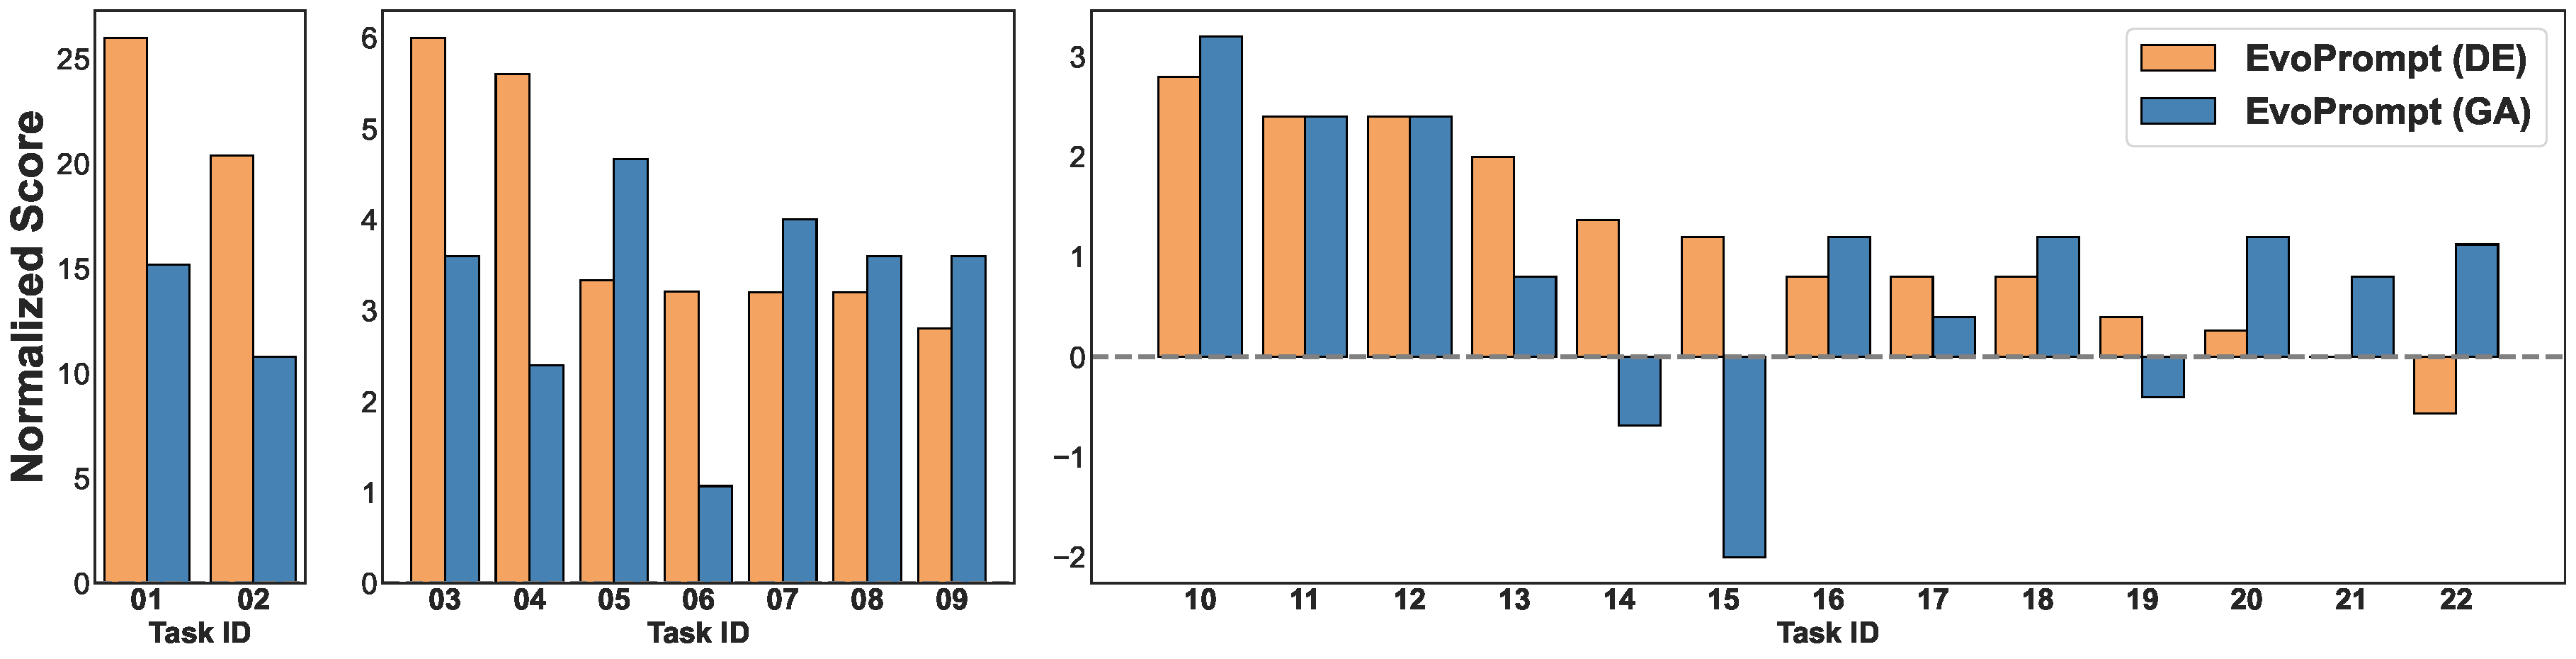
\includegraphics[width=\textwidth]{images/bbh.pdf}
    \caption{Normalized scores on BBH tasks for \modelname (GA) and \modelname (DE). }
    \label{fig:exp-bbh}
\end{figure}